\newpage
\section{Technologierecherche}

Anforderungen in Teilfunktionen zerlegt:
\begin{itemize}
    \item Fortbewegung
    \item Antrieb
    \item Steuerung
    \item Orientierung
    \item Bilderkennung
    \item Wegselektierung
    \item Sicherheit
    \item Energiequelle
    \item Hindernis Bewältigung
    \item 
\end{itemize}

\subsection*{Überblick}

\scriptsize
\begin{longtable}{l@{\extracolsep{\fill}}p{2cm}p{2cm}p{4cm}p{1.5cm}lll}
%\toprule
\textbf{Dep.} & \textbf{Teilfunktion} & \textbf{Thema} &
\textbf{Beschreibung} & \textbf{Bewertung (0-10)} & \textbf{Quelle} & \textbf{Abfragedatum} &
\textbf{Wer}\tabularnewline
%\midrule
\endhead

M & Fortbewegung & Beweglichkeit & 2-Rad gegensinnig für 360° \newline Drehung im Stand & 8 & MC-Car & 01.10.2024 & Joel
\tabularnewline
M & Fortbewegung & Beweglichkeit & 4-Rad Differential steering / \newline skid steer & 8 & \href{https://en.wikipedia.org/wiki/Differential_steering}{Link} /\href{https://science.howstuffworks.com/transport/engines-equipment/skid-steer2.htm}{Link} & 03.10.2024 & Silas
\tabularnewline
M & Fortbewegung & Beweglichkeit & Omniwheels & 9 & \href{https://de.wikipedia.org/wiki/Allseitenrad}{Link} / \href{https://www.youtube.com/watch?v=wwQQnSWqB7A}{Link} & 03.10.2024 & Silas
\tabularnewline
M & Fortbewegung & Beweglichkeit & Knicklenkung & 4 & \href{https://de.wikipedia.org/wiki/Knicklenkung}{Link} & 03.10.2024 & Silas
\tabularnewline
M & Fortbewegung & Beweglichkeit & Achsschenkellenkung & 5 & \href{https://de.wikipedia.org/wiki/Achsschenkel#:~:text=Die%20Erfindung%20der%20Achsschenkellenkung%20bedeutete,wird%20bei%20Automobilen%20ausschlie%C3%9Flich%20verwendet.}{Link} & 03.10.2024 & Silas
\tabularnewline
M & Fortbewegung & Beweglichkeit & Drehschemellenkung & 5 & \href{https://www.staplerberater.de/auswahlkriterien/lenkungsarten}{Link} & 03.10.2024 & Silas
\tabularnewline
M & Fortbewegung & Beweglichkeit & Fahrzeug abbocken und an Stelle auf Drehkranz wenden & 6 & \href{https://www.kaiserkraft.ch/hubgeraete/hub-und-verladetische/auto-niveaugeraet-mit-drehscheibe/drehscheiben-1110-mm/p/M1142876/?articleNumber=118558&lang=de_CH&customerType=B2C&lang=&infinity=ict2~net~gaw~cmp~PM_DE-shopping24-Jarvis-0~ag~~ar~~kw~~mt~&gad_source=1&gclid=CjwKCAjwgfm3BhBeEiwAFfxrGxsQhJoEWwY3dNM_OYKFg2NOgoHXLP2OeyLmOZFTVnzHt7PvNpgCbhoCACQQAvD_BwE}{Link} & 03.10.2024 & Silas
\tabularnewline

E & Antrieb & Motor & Schrittmotor & 8 & \href{https://wiki.bu.ost.ch/infoportal/_media/hardware/sysp/bauteile/schrittmotor_kurz_erklaert_d.pdf}{Link} & 27.09.2024 & Thomas
\tabularnewline
E & Antrieb & Motor & DC Motor & 7 & \href{https://www.elektronikpraxis.de/dc-motoren-empirisch-und-theoretisch-berechnen-a-04bb230e718c01ace9dd584576d618a3/}{Link} & 27.09.2024 & Thomas
\tabularnewline
E & Antrieb & Motor & Brushless & 7 & \href{https://www.renesas.com/en/support/engineer-school/brushless-dc-motor-01-overview}{Link} & 27.09.2024 & Thomas
\tabularnewline

I & Steuerung & Hardware & Raspberry Pi & 8 & \href{https://www.raspberrypi.com/documentation/computers/raspberry-pi.html}{Link} & 29.09.2024 & Thomas
\tabularnewline
I & Steuerung & Hardware & Arduino & 5 & \href{https://arduino.cc/en/hardware#boards-1}{Link} & 29.09.2024 & Thomas
\tabularnewline
I & Steuerung & Hardware & Tiny & 8 & HSLU & 01.10.2024 & Joel
\tabularnewline
I & Steuerung & Hardware & ESP32 & 7 & \href{https://www.espressif.com/en/products/devkits/esp32-devkitc}{Link} & 03.10.2024 & Thomas
\tabularnewline

E & Orientierung & Sensorik & Infrarot & 5 & \href{https://www.elektronik-kompendium.de/sites/raspberry-pi/2802011.htm}{Link} & 27.09.2024 & Thomas
\tabularnewline
E & Orientierung & Sensorik & Ultraschall & 5 & \href{https://elektro.turanis.de/html/prj121/index.html}{Link} & 27.09.2024 & Thomas 
\tabularnewline
E & Orientierung & Sensorik & Encoder & 7 & \href{https://www.arrow.de/research-and-events/articles/rotary-encoders-how-to-pair-with-an-arduino-board}{Link} & 29.09.2024 & Thomas
\tabularnewline
E & Orientierung & Sensorik & Optischer Sensor & 5 & \href{https://global.sharp/products/device/lineup/data/pdf/datasheet/gp2y0e02a_e.pdf}{Link} & 01.10.2024 & Joel
\tabularnewline

I &  Objekterkennung &  Deep Learning & Deep Learning Frameworks & 7 &  \href{https://www.simplilearn.com/tutorials/deep-learning-tutorial/deep-learning-frameworks} {Link}&  27.09.2024 & Gian
\tabularnewline
I & Objekterkennung & Deep Learning & TensorFlow in 100 seconds & 10 &
\href{https://www.youtube.com/watch?v=i8NETqtGHms}{Link} & 29.09.2024 & Gian
\tabularnewline


I & Wegfindung & Algorithmus & Informationen über Wegfindung & \href{https://de.wikipedia.org/wiki/Pathfinding}{Link} & 8 & 02.10.2024 & Gian
\tabularnewline
I & Wegfindung & Test & Test & Test & Test & Test & Test
\tabularnewline
I & Wegfindung & Test & Test & Test & Test & Test & Test
\tabularnewline

E & Sicherheit & Not-Aus & Implementierung eines Not-Aus & 6 & \href{https://www.eaton.com/ie/en-gb/markets/machine-building/service-and-support-machine-building-moem-service-eaton/blogs/emergency-stop-circuit---blogs---eaton.html}{Link} & 27.09.2024 & Thomas
\tabularnewline
E & Sicherheit & Sicherheit & Sicherheit mobiler Roboter & 5 & \href{https://tuprints.ulb.tu-darmstadt.de/18674/1/10.1524_auto.51.10.435.19576.pdf}{Link} & 27.09.2024 & Thomas 
\tabularnewline

E & Energiequelle & Akkumulatoren & LiPo & 8 & \href{https://www.lion-care.com/lipo-akkus-eigenschaften-vorteile-und-mehr}{Link} & 27.09.2024 & Thomas
\tabularnewline
E & Energiequelle & Akkumulatoren & Li-Ion & 7 & \href{https://poleenergy.ch/shop_content.php?coID=32}{Link} & 27.09.2024 & Thomas
\tabularnewline
E & Energiequelle & Solarpanel & Run Arduino Offgrid & 6 & \href{https://voltaicsystems.com/solar-arduino-guide/}{Link} & 29.09.2024 & Thomas
\tabularnewline
E & Energiequelle & Akkumulatoren & Nickel-Metallhydrid-Akkus \newline (Batterie) & 7 & \href{https://voltaicsystems.com/solar-arduino-guide/}{Link} & 29.09.2024 & Joel
\tabularnewline

M & Hindernissbewältigung & Aufnahme & gegen Fahrzeug pressen & 8 &  & 03.10.2024 & Silas
\tabularnewline
M & Hindernissbewältigung & Aufnahme & Palettengabel in Löcher von Hindernis  & 5 &  & 03.10.2024 & Silas
\tabularnewline
M & Hindernissbewältigung & Aufnahme & Vakuumgreifer & 5 & \href{https://www.schmalz.com/de-ch/glossar/vakuumgreifer/}{Link} & 03.10.2024 & Silas
\tabularnewline
M & Hindernissbewältigung & Transport & ganzes Fahrzeug wenden & 8 &  & 03.10.2024 & Silas
\tabularnewline
M & Hindernissbewältigung & Transport & über Fahrzeug hinweg mit Ausleger & 6 &  & 03.10.2024 & Silas
\tabularnewline
M & Hindernissbewältigung & Transport & über Fahrzeug hinweg mit Förderband & 3 &  & 03.10.2024 & Silas
\tabularnewline


\caption{Technologierecherche Übersicht}
\label{tab:technologierecherche}
\end{longtable}
\normalsize

\newpage
\subsection{Informatik}

Dieser Abschnitt enthält detaillierte Rechercheergebnise über die Bereiche der Informatik.

\subsubsection{Wegfindung}

Die Topologie des Weges mit Start und Zielmöglichkeiten ist bereits bekannt.
Somit kann anhand eines Wegfindungsalgorithmus der schnellste Weg berechnet werden.

\paragraph{Dijkstra}

Findet den kürzesten Weg von einem gegebenen Startknoten zu allen anderen Knoten in einem Graphen mit nicht-negativen Gewichten.

\begin{multicols}{2}
\begin{items}
  \item [Vorteile]
  \item Optimierter Greedy-Algorithmus, der immer die optimale Lösung findet.
\end{items}

\columnbreak

\begin{items}
  \item [Nachteile]
  \item Nicht zielgerichtet, kann zu Zeitverschwendung führen
\end{items}
\end{multicols}

\subsubsection{Linienerkennung}

Der anhand von Linien eingezeichnete Weg muss erkannt werden.
Die verschiedenen Möglichkeiten werden hier aufgelistet.

\subsubsection{Objekterkennung}

Die Hindernisse sowie die Pylonen müssen anhand von Software erkannt und kategorisiert werden.
Um die beiden Objekte voneinenader zu unterscheiden, müssen die Objekte anhand von Bildern erkannt werden.

\begin{tabular}{|p{5cm}|l|l|}
\hline
\textbf{Framework} & \textbf{Beschreibung} & \textbf{Something}
\\ \hline
TensorFlow
& Test & Test
\\ \hline
Scikit-learn & Test & Test
\\ \hline
\end{tabular}

\subsubsection{Simulation}


\newpage
\subsection{Hindernis Bewältigung}
Folgendes sind Ideen für die Hindernisbewältigung, jeweils mit einer Skizze oder Quelle. Die Aufgabe wurde in den Teil Aufnahme des Hindernisses und Rotation / Transport unterteilt.
\subsubsection{Aufnahme Hindernis}
\begin{figure}[h!]
    \centering
    \begin{minipage}{0.45\textwidth}
        \centering
        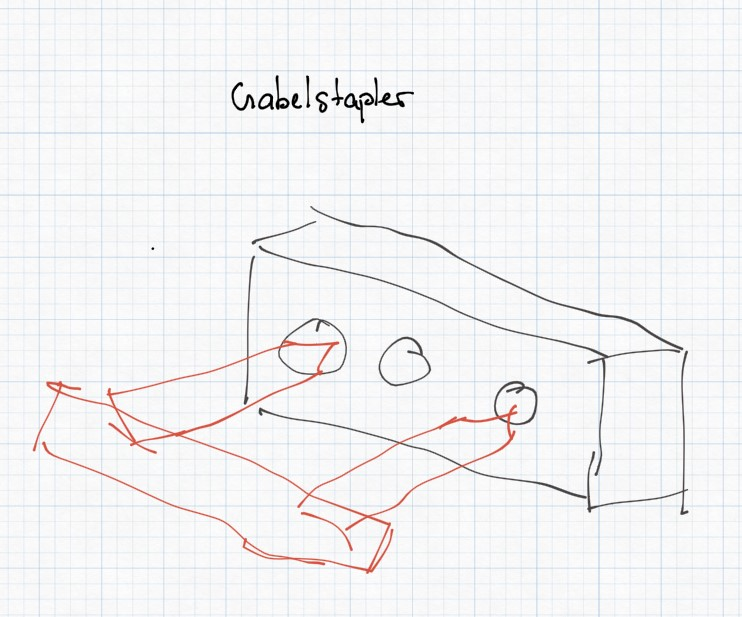
\includegraphics[width=\textwidth]{img/technologierecherche/Aufnahme/Gabelstapler.jpg}
        \caption{Prinzip angelehnt an einen Gabelstapler}
        \label{img:tech_Gaplerstapler}
    \end{minipage}
    \hfill
    \begin{minipage}{0.45\textwidth}
        \centering
        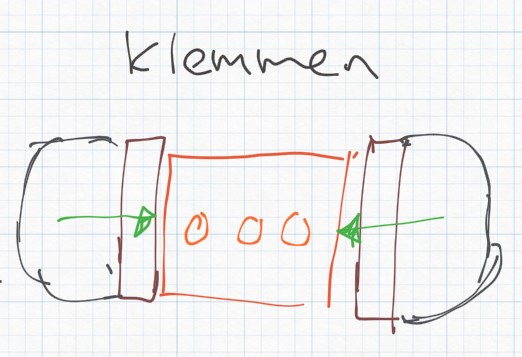
\includegraphics[width=\textwidth]{img/technologierecherche/Aufnahme/Laengsweg_Griff.jpg}
        \caption{Klemme über Längsweg des Hindernisses}
        \label{img:tech_Laengsweg_Griff}
    \end{minipage}
\end{figure}
\newpage
\begin{figure}[h!]
    \centering
    \begin{minipage}{0.45\textwidth}
        \centering
        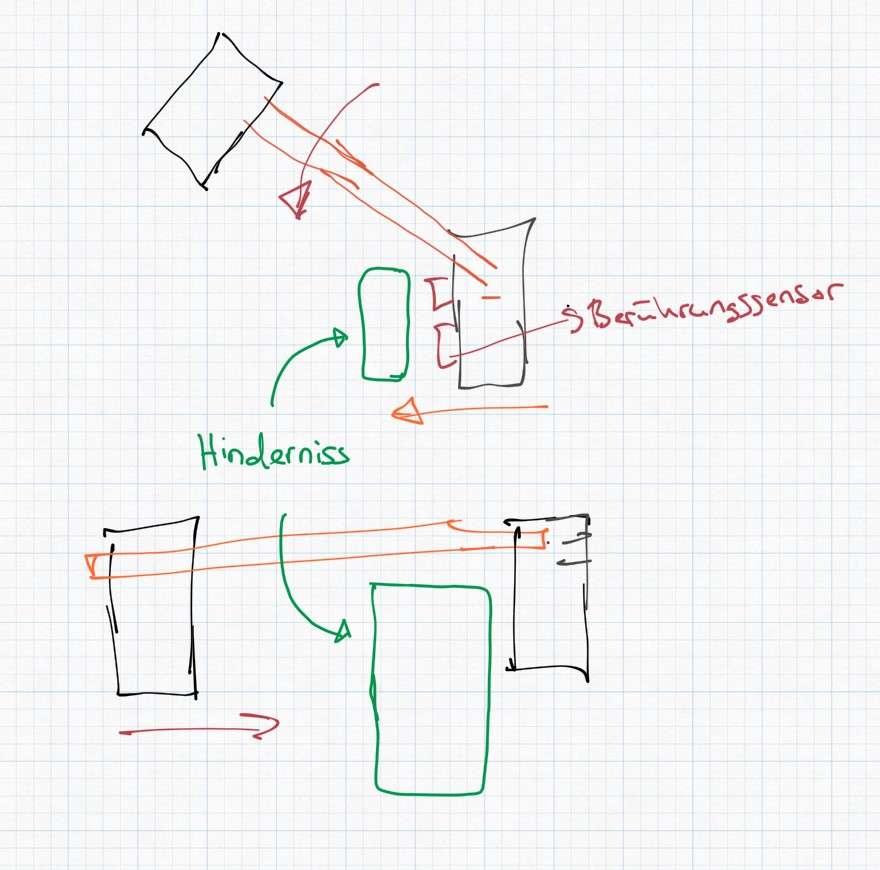
\includegraphics[width=\textwidth]{img/technologierecherche/Aufnahme/Breiterweg_Griff.jpg}
        \caption{Klemme über Breitenweg des Hindernisses, kann modifiziert werden, um Berührungssensoren zu verwenden}
        \label{img:tech_Breiterweg_Griff}
    \end{minipage}
    \hfill
    \begin{minipage}{0.45\textwidth}
        \centering
        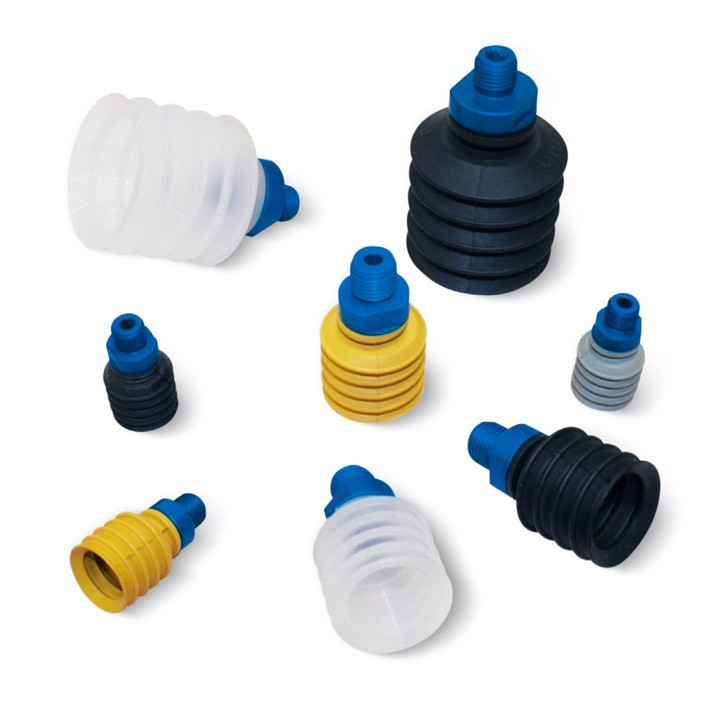
\includegraphics[width=\textwidth]{img/technologierecherche/Aufnahme/Vakuumgreifer.jpg}
        \caption{Aufnahme über Vakuumgreifer, Quelle: https://www.youtube.com/shorts/alxwWgzSVss} 
        \label{img:tech_Vakuumgreifer}
    \end{minipage}
\end{figure}


\newpage
\subsubsection{Rotation / Transport}
\begin{figure}[h!]
    \centering
    \begin{minipage}{0.45\textwidth}
        \centering
        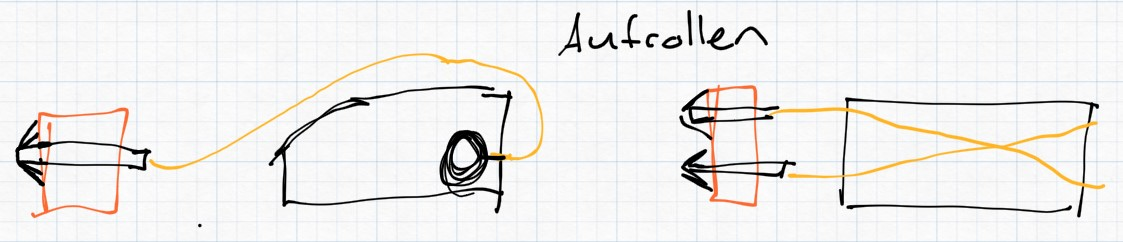
\includegraphics[width=\textwidth]{img/technologierecherche/Rotation/harponne.jpg}
        \caption{Eine Harpune artige Konstruktion, die die Löcher des Hindernisses ausnutzt}
        \label{img:tech_harponne}
    \end{minipage}
    \hfill
    \begin{minipage}{0.45\textwidth}
        \centering
        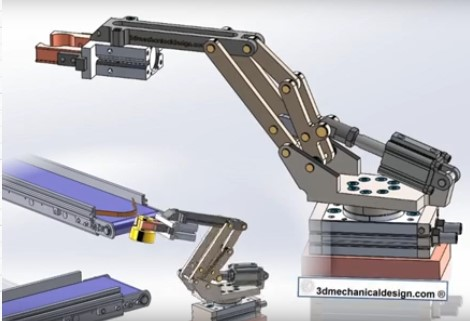
\includegraphics[width=\textwidth]{img/technologierecherche/Rotation/kran.jpg}
        \caption{Eine an einen Kran angelegte Konstruktion, Quelle: https://www.youtube.com/watch?v=VZRFHJfUkq4\&feature=youtu.be} 
        \label{img:tech_kran}
    \end{minipage}
\end{figure}

\begin{figure}[h!]
    \centering
    \begin{minipage}{0.45\textwidth}
        \centering
        \includegraphics[width=\textwidth]{img/technologierecherche/Rotation/seitlich_mit_räder.jpg}
        \caption{Für die Rotation wird das ganze Fahrzeug gewendet}
        \label{img:tech_seitlich_mit_räder}
    \end{minipage}
    \hfill
    \begin{minipage}{0.45\textwidth}
        \centering
        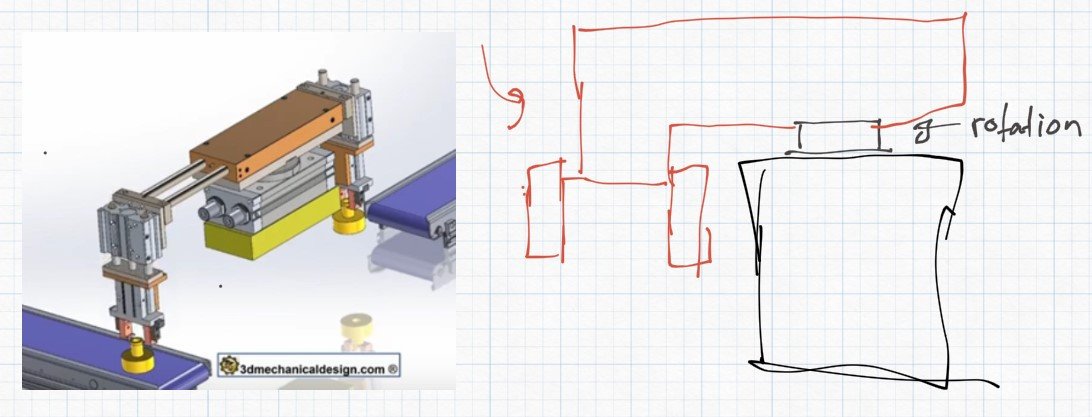
\includegraphics[width=\textwidth]{img/technologierecherche/Rotation/seitlich_mit_rotation.jpg}
        \caption{Ebenfalls an einen Kran angelegt, jedoch wird die Aufnahme von oben auf die Breite des Fahrzeuges durchgeführt, Quelle:https://www.youtube.com/watch?v=J7LGSNhFTU4} 
        \label{img:tech_seitlich_mit_rotation}
    \end{minipage}
\end{figure}
\newpage
\begin{figure}[h!]
    \centering
    \begin{minipage}{0.45\textwidth}
        \centering
        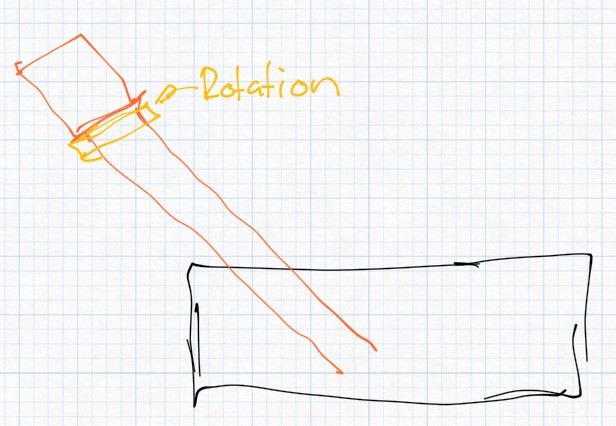
\includegraphics[width=\textwidth]{img/technologierecherche/Rotation/ueberkopf_griff_gelagert.jpg}
        \caption{}
        \label{img:tech_ueberkopf_griff_gelagert}
    \end{minipage}
    \hfill
    \begin{minipage}{0.45\textwidth}
        \centering
        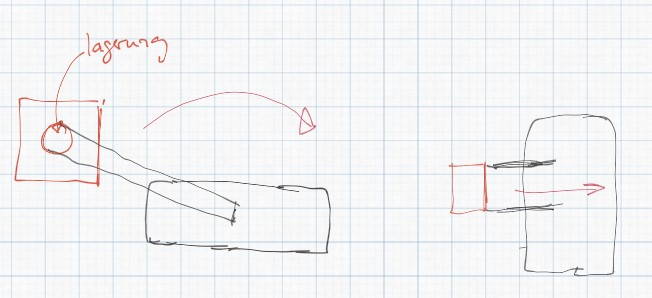
\includegraphics[width=\textwidth]{img/technologierecherche/Rotation/ueberkopf_objekt_gelagert.jpg}
        \caption{} 
        \label{img:tech_ueberkopf_objekt_gelagert}
    \end{minipage}
\end{figure}

\begin{figure}[h!]
    \centering
    \begin{minipage}{0.45\textwidth}
        \centering
        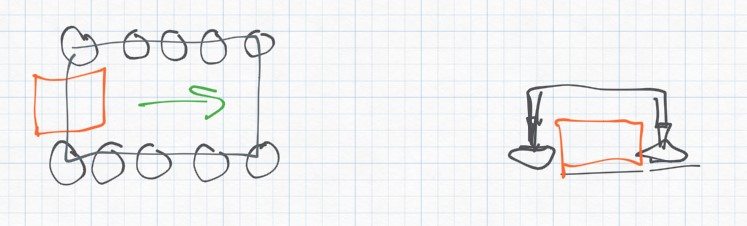
\includegraphics[width=\textwidth]{img/technologierecherche/Rotation/waescheanlage.jpg}
        \caption{}
        \label{img:tech_waescheanlage}
    \end{minipage}
    \hfill
    \begin{minipage}{0.45\textwidth}
        \centering
        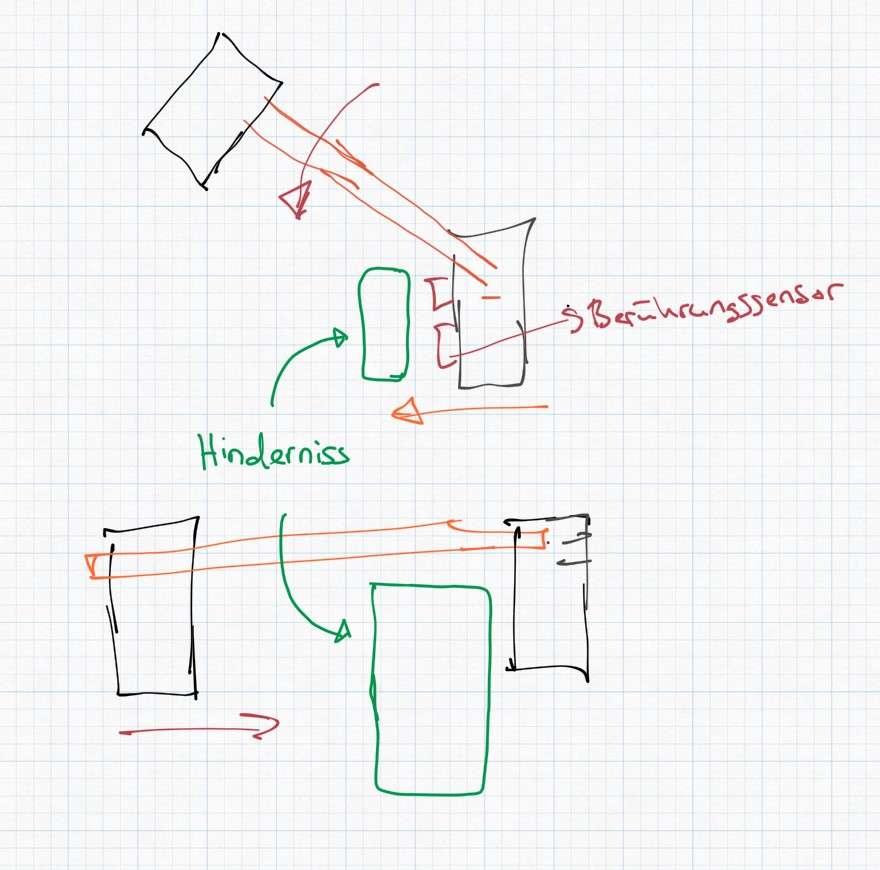
\includegraphics[width=\textwidth]{img/technologierecherche/Aufnahme/Breiterweg_Griff.jpg}
        \caption{} 
        \label{img:tech_nichts}
    \end{minipage}
\end{figure}
